\chapter{Captura de requisitos}
%\newpage
%Que tiene que cumplir el trabajo que se va a desarrollar, 
%que necesidades tiene que satisfacer, quienes van a ser sus usuarios, etc.
%
%En un trabajo de desarrollo de software tradicional se 
%documentará mediante el Modelo de casos de uso y la jerarquía 
%de actores, acompañando cada caso de uso y cada actor de una pequeña definición.

\section{Diagrama de casos de uso}
En el diagrama de casos de uso, se puede ver qu\'e acciones puede realizar el 
usuario en cualquier momento, y cuales
est\'an supeditadas a ciertas condiciones. N\'otese que las condiciones de los ``extend" \ son los comentarios a\~nadidos
a los subcasos de uso.

Los casos de uso extendidos se encuentran en el anexo \ref{chap:CasosDeUsoExt}

\begin{figure}[h]
\centering
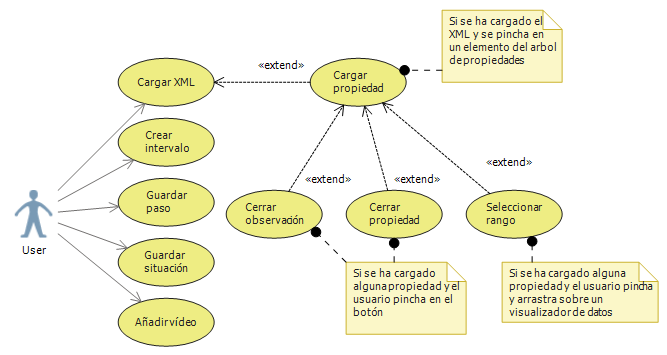
\includegraphics[width=1.0\linewidth]{./Figures/useCaseDiagram.png}
\caption[Diagrama de casos de uso]{Diagrama de casos de uso}
\label{fig:useCaseDiagram}
\end{figure}

\subsection{Cargar XML}
Carga un XML que contiene las propiedades y las observaciones en el sistema.
\'Unicamente se cargan si el fichero valida contra el XSD.

\subsection{A\~nadir v\'ideo}
Abre un v\'ideo y lo a\~nade al contenedor de v\'ideos si ya hab\'ia alguno 
cargado previamente. Si no, a\~nade tambi\'en un contenedor de v\'ideos.

\subsection{Cargar propiedad}
Carga una propiedad en el contenedor de gr\'aficos correspondiente a la observaci\'on a la que pertenece.
Tambi\'en se pueden a\~nadir propiedades en grupo, haciendo doble click sobre el nombre de la observaci\'on.
Si el contenedor de esa observaci\'on o propiedad no est\'a creado, lo crea.

\subsection{Seleccionar rango}
Al pinchar y mover el rat\'on sobre un visualizador de datos, se seleccionar\'a ese rango en todos
los visualizadores de datos cargados en el sistema.

\subsection{Cerrar observaci\'on}
Elimina, tanto de la interfaz gr\'afica como de memoria, la observaci\'on
seleccionada y todos sus visualizadores de datos (propiedades) asociadas.

\subsection{Cerrar propiedad}
Elimina, tanto gr\'aficamente, como de memoria, la propiedad seleccionada.

\subsection{Crear intervalo}
A\~nade el intervalo seleccionado a los intervalos a guardar en el XML si no se superpone con los que
ya est\'an guardados.

\subsection{Guardar paso}
Guarda todos los intervalos creados a disco con un elemento ra\'iz ``step".

\subsection{Guardar situaci\'on}
Guarda todos los intervalos creados a disco con un elemento ra\'iz ``situation".



\section{Modelo de dominio}
La Figura \ref{fig:ModelodeDominio} representa tanto los datos de entrada del software, tanto los datos
de salida.

\begin{figure}[H]
\centering
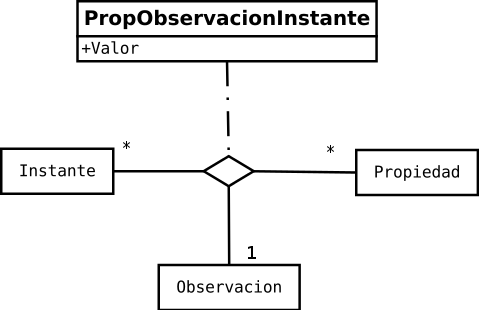
\includegraphics[width=0.7\linewidth]{./Figures/ModelodeDominio}
\caption[Modelo de dominio]{Modelo de dominio}
\label{fig:ModelodeDominio}
\end{figure}

\subsection{Observaci\'on}
La entidad observaci\'on la compone una lista propiedades y un nombre \'unico, que describe la observaci\'on,
por ejemplo ``pelota en movimiento".

\subsection{Propiedad}
Las propiedades est\'an formadas por una serie de instantes, y un nombre de propiedad, que detalla el
significado de la propiedad, por ejemplo, ``velocidad".

\subsection{Instante}
Los instantes se componen de un atributo ``instante de simulaci\'on", que indica en que instante est\'a sucediendo
dicho Instante.

\subsection{PropObservacionInstante}
Tal y como se ve en la Figura \ref{fig:ModelodeDominio} para una observaci\'on y una propiedad,
hay muchos instantes, para un instante concreto y una observaci\'on 
hay m\'ultiples propiedades, y para
una propiedad y un instante, hay una \'unica observaci\'on.

Podr\'ia pensarse en no utilizar una relaci\'on ternaria, sino dos binarias.
Para explicar porque no puede ser, lo mejor es utilizar un ejemplo. Supongamos que tenemos las
observaciones Obs1 y Obs2, as\'i como las propiedad Prop1, Prop2 y Prop3, y los instantes Ins1, Ins2.

Obs1 contiene: Prop1 y Prop3.
Obs2 contiene: Prop1 y Prop2.

N\'otese que las propiedades aunque tengan el mismo nombre, no son la misma propiedad si est\'an en observaciones distintas.
Llegados a este punto, estar\'iamos incumpliendo una de las restricciones del modelo de dominio, que dice que en una
relaci\'on binaria, una pareja de datos solo puede darse una vez, y es factible pensar que existir\'a tanto
(Prop1, Ins1) para la Obs1 como para la Obs2.

Como esa restricci\'on no puede incumplirse, se utiliza una relaci\'on ternaria, en la que se tiene la certeza
que la tripleta (Obs1, Prop1, Ins1) no va a repetirse. Finalmente, para esa tripleta se guarda el valor que se ha
seleccionado.